\documentclass[journal,12pt,twocolumn]{IEEEtran}

\usepackage{setspace}
\usepackage{gensymb}

\singlespacing


\usepackage[cmex10]{amsmath}

\usepackage{amsthm}

\usepackage{mathrsfs}
\usepackage{txfonts}
\usepackage{stfloats}
\usepackage{bm}
\usepackage{cite}
\usepackage{cases}
\usepackage{subfig}

\usepackage{longtable}
\usepackage{multirow}

\usepackage{enumitem}
\usepackage{mathtools}
\usepackage{steinmetz}
\usepackage{tikz}
\usepackage{circuitikz}
\usepackage{verbatim}
\usepackage{tfrupee}
\usepackage[breaklinks=true]{hyperref}
\usepackage{graphicx}
\usepackage{tkz-euclide}
\usepackage{float}

\usetikzlibrary{calc,math}
\usepackage{listings}
    \usepackage{color}                                            %%
    \usepackage{array}                                            %%
    \usepackage{longtable}                                        %%
    \usepackage{calc}                                             %%
    \usepackage{multirow}                                         %%
    \usepackage{hhline}                                           %%
    \usepackage{ifthen}                                           %%
    \usepackage{lscape}     
\usepackage{multicol}
\usepackage{chngcntr}

\DeclareMathOperator*{\Res}{Res}

\renewcommand\thesection{\arabic{section}}
\renewcommand\thesubsection{\thesection.\arabic{subsection}}
\renewcommand\thesubsubsection{\thesubsection.\arabic{subsubsection}}

\renewcommand\thesectiondis{\arabic{section}}
\renewcommand\thesubsectiondis{\thesectiondis.\arabic{subsection}}
\renewcommand\thesubsubsectiondis{\thesubsectiondis.\arabic{subsubsection}}


\hyphenation{op-tical net-works semi-conduc-tor}
\def\inputGnumericTable{}                                 %%

\lstset{
%language=C,
frame=single, 
breaklines=true,
columns=fullflexible
}
\begin{document}


\newtheorem{theorem}{Theorem}[section]
\newtheorem{problem}{Problem}
\newtheorem{proposition}{Proposition}[section]
\newtheorem{lemma}{Lemma}[section]
\newtheorem{corollary}[theorem]{Corollary}
\newtheorem{example}{Example}[section]
\newtheorem{definition}[problem]{Definition}

\newcommand{\BEQA}{\begin{eqnarray}}
\newcommand{\EEQA}{\end{eqnarray}}
\newcommand{\define}{\stackrel{\triangle}{=}}
\bibliographystyle{IEEEtran}
\providecommand{\mbf}{\mathbf}
\providecommand{\pr}[1]{\ensuremath{\Pr\left(#1\right)}}
\providecommand{\qfunc}[1]{\ensuremath{Q\left(#1\right)}}
\providecommand{\sbrak}[1]{\ensuremath{{}\left[#1\right]}}
\providecommand{\lsbrak}[1]{\ensuremath{{}\left[#1\right.}}
\providecommand{\rsbrak}[1]{\ensuremath{{}\left.#1\right]}}
\providecommand{\brak}[1]{\ensuremath{\left(#1\right)}}
\providecommand{\lbrak}[1]{\ensuremath{\left(#1\right.}}
\providecommand{\rbrak}[1]{\ensuremath{\left.#1\right)}}
\providecommand{\cbrak}[1]{\ensuremath{\left\{#1\right\}}}
\providecommand{\lcbrak}[1]{\ensuremath{\left\{#1\right.}}
\providecommand{\rcbrak}[1]{\ensuremath{\left.#1\right\}}}
\theoremstyle{remark}
\newtheorem{rem}{Remark}
\newcommand{\sgn}{\mathop{\mathrm{sgn}}}
\providecommand{\abs}[1]{\left\vert#1\right\vert}
\providecommand{\res}[1]{\Res\displaylimits_{#1}} 
\providecommand{\norm}[1]{\left\lVert#1\right\rVert}
%\providecommand{\norm}[1]{\lVert#1\rVert}
\providecommand{\mtx}[1]{\mathbf{#1}}
\providecommand{\mean}[1]{E\left[ #1 \right]}
\providecommand{\fourier}{\overset{\mathcal{F}}{ \rightleftharpoons}}
%\providecommand{\hilbert}{\overset{\mathcal{H}}{ \rightleftharpoons}}
\providecommand{\system}{\overset{\mathcal{H}}{ \longleftrightarrow}}
	%\newcommand{\solution}[2]{\textbf{Solution:}{#1}}
\newcommand{\solution}{\noindent \textbf{Solution: }}
\newcommand{\cosec}{\,\text{cosec}\,}
\providecommand{\dec}[2]{\ensuremath{\overset{#1}{\underset{#2}{\gtrless}}}}
\newcommand{\myvec}[1]{\ensuremath{\begin{pmatrix}#1\end{pmatrix}}}
\newcommand{\mydet}[1]{\ensuremath{\begin{vmatrix}#1\end{vmatrix}}}
\numberwithin{equation}{subsection}
\makeatletter
\@addtoreset{figure}{problem}
\makeatother
\let\StandardTheFigure\thefigure
\let\vec\mathbf
\renewcommand{\thefigure}{\theproblem}
\def\putbox#1#2#3{\makebox[0in][l]{\makebox[#1][l]{}\raisebox{\baselineskip}[0in][0in]{\raisebox{#2}[0in][0in]{#3}}}}
     \def\rightbox#1{\makebox[0in][r]{#1}}
     \def\centbox#1{\makebox[0in]{#1}}
     \def\topbox#1{\raisebox{-\baselineskip}[0in][0in]{#1}}
     \def\midbox#1{\raisebox{-0.5\baselineskip}[0in][0in]{#1}}
\vspace{3cm}
\title{Assignment 6}
\author{K.A. Raja Babu}
\maketitle
\newpage
\bigskip
\renewcommand{\thefigure}{\theenumi}
\renewcommand{\thetable}{\theenumi}
Download all python codes from 
\begin{lstlisting}
https://github.com/ka-raja-babu/Matrix-Theory/tree/main/Assignment6/Codes
\end{lstlisting}
%
and latex-tikz codes from 
%
\begin{lstlisting}
https://github.com/ka-raja-babu/Matrix-Theory/tree/main/Assignment6
\end{lstlisting}
%
\section{Question No. 2.29}
Find the coordinates of the focus, axis, the equation of the directrix and latus rectum of the parabola $y^2$ = 8$x$ .
%
\section{Solution}
\numberwithin{table}{section}
\begin{table}[!ht]
\begin{center}
\begin{tabular}{ | m{1.4cm} | m{1.0cm}| m{2.4cm} | m{2.3cm} | } 
\hline
Para-\newline meter  & Sym-\newline bol  & Value  & General \newline Formula\\ 
\hline
Vertex & $\vec{c}$ & $\myvec{0\\0}$ & $\myvec{\vec{u}^T + \eta\vec{p_1}^T \\ \vec{V}}\vec{c}$ \newline $= \myvec{-f \\ \eta\vec{p_1} - \vec{u}}$ \\ 
\hline
Focal \newline Length & $\beta$ & 2 & $\frac{1}{4}\abs{\frac{2\eta}{\lambda_2}}$
\\ 
\hline
Focus & $\vec{F}$ & \myvec{2\\0} & $\vec{F}=\vec{c} + \vec{a}^T$ \\
\hline
Axis &  & $\myvec{0 & 1}\vec{x}=0$ & $\vec{x}=\vec{F}+k\vec{m}$ \\
\hline
Direct- \newline rix & & $\myvec{1 & 0}\vec{x} = -2$ & $\vec{v_1}\vec{x} = -\beta$ \\
\hline
Latus \newline rectum & & $\myvec{1 & 0}\vec{x}=2$ & $\vec{v_2}\vec{x}=\beta$\\
\hline
End \newline points \newline of latus \newline rectum & $\vec{M},\vec{N}$ & $\myvec{2\\4},\myvec{2\\-4}$ & $\myvec{\beta \\ \pm y(\beta)}$ \\
\hline
Length \newline of latus \newline rectum & $l$ & 8 & $\norm{\vec{M}-\vec{N}}$\\
\hline
\end{tabular}
\end{center}
\caption{Parameters of parabola}
\label{tab:table1}
\end{table}

All parameters of parabola can be summarised in table \ref{tab:table1}

Note : Given general formula is valid only when parabola is in standard form i.e. $\abs{\vec{V}}$ = 0 and $\lambda_1$ = 0 . 

Given parabola is 
\begin{align}
y^2 &= 8x
\\
\implies y^2 - 8x &= 0
\end{align}

Vector form of given parabola is
\begin{align}
\vec{x}^T\myvec{0 & 0 \\ 0 & 1}\vec{x} + 2\myvec{-4 & 0}\vec{x} + 0 &= 0 
\end{align}

$\therefore$
\begin{align}
 \vec{V} = \myvec{0 & 0 \\ 0 & 1} ,
 \vec{u} = \myvec{-4\\0} ,
 f = 0
\end{align}

$\because$
$|\vec{V}|$ = 0 and $\lambda_1$ = 0 i.e. it is in standard form
\\
$\therefore$
\begin{align}
\vec{P}=\vec{I} \implies \vec{p_1} = \myvec{1\\0}
\\
\eta = \vec{u}^T\vec{p_1} = -4
\end{align}

The vertex $\vec{c}$ is given by
\begin{align}
\myvec{-8 & 0\\0 & 0\\0 & 1}\vec{c} &= \myvec{0\\0\\0}
\\
\implies \vec{c} &= \myvec{0\\0}
\end{align}

The focal length $\beta$ is given by
\begin{align}
\beta = \frac{1}{4}\abs{\frac{2\eta}{\lambda_2}} = \frac{1}{4}\abs{\frac{-8}{1}}= 2
\end{align}

The focus $\vec{F}$ is given by
\begin{align}
\vec{a} &= \frac{-2\eta\myvec{1 & 0}}{4} = \myvec{2 & 0}
\\
\vec{F} &= \vec{c} + \vec{a}^T = \myvec{2\\0}
\end{align}

$\because$
Axis of parabola passes through both vertex and focus .
\\
$\therefore$
Axis of parabola is given by
\begin{align}
\vec{m} =\vec{F} - \vec{c} &= \myvec{2\\0}
\\
\vec{x} = \vec{F} + k\vec{m} &= \myvec{2+2k \\ 0}
\\
\implies \myvec{0 & 1}\vec{x} &= 0
\end{align}

$\because$
Vertex of parabola is at equal distance from focus and directrix and is perpendicular to axis.
\\
$\therefore$
Directrix of parabola is given by
\begin{align}
\myvec{0 & 1}\vec{v_1}^T = 0
\\
\implies \vec{v_1} = \myvec{1 & 0}
\end{align}
So , 
\begin{align}
\vec{v_1}\vec{x} = -\beta
\\
\implies \myvec{1 & 0}\vec{x} = -2
\end{align}

$\because$
Latus rectum of parabola passes through focus and is perpendicular to axis.
\\
$\therefore$
Latus rectum of parabola is given by
\begin{align}
\myvec{0 & 1}\vec{v_2}^T = 0
\\
\implies \vec{v_2} = \myvec{1 & 0}
\end{align}
So , 
\begin{align}
\vec{v_2}\vec{x} = \beta
\\
\implies \myvec{1 & 0}\vec{x} = 2
\end{align}

End points of latus rectum are
\begin{align}
\vec{M} &= \myvec{2\\4}
\\
\vec{N} &= \myvec{2\\-4}
\end{align}

So,the length of latus rectum $l$ is 
\begin{align}
l = \norm{\vec{M}-\vec{N}} = 8
\end{align}

\newpage
Plot of given parabola

\numberwithin{figure}{section}
\begin{figure}[!ht]
\centering
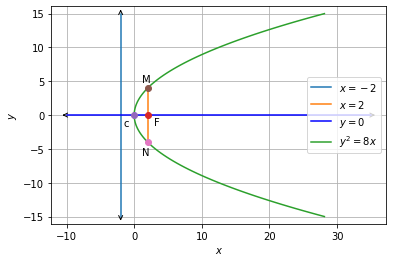
\includegraphics[width=\columnwidth]{Figure6}
\caption{Parabola $y^2=8x$ }
\label{fig:parabola}	
\end{figure}

\end{document}
